\chapter{Methodik}
\label{chap:methodik}

Dieses Kapitel beschreibt, wie die Forschungsfragen bearbeitet werden.

\section{Versuchsaufbau}
\label{sec:aufbau}

Abbildung~\ref{fig:pipeline} zeigt den Versuchsaufbau. In dieser Arbeit wird jedes Bild auf $224\times224$ Pixel skaliert und mit den Mittelwerten und den Standardabweichungen von ImageNet normiert. DINOv2 ViT-B/14 überführt es anschließend in seinen \ac{CLS}-Merkmalsvektor $\bm{\varphi}_i$ mit 768 Dimensionen~\cite{oquab_dinov2_2023}. Auf $224\times224$ Pixel skaliert auch die Studie zum Training von Retrieval-Modellen~\cite{berton_all_2025}. In dieser Arbeit bleibt das Backbone dagegen eingefroren. Die Merkmale werden einmal berechnet und gespeichert. Trainiert wird nur ein linearer Projection Head. Das normierte Embedding eines Bildes lautet
\begin{equation}
  \bm{f}_i=\frac{\bm{A}\bm{\varphi}_i+\bm{b}}{\lVert\bm{A}\bm{\varphi}_i+\bm{b}\rVert_2},\qquad \bm{A}\in\mathbb{R}^{768\times768},\ \bm{b}\in\mathbb{R}^{768},
  \label{eq:kopf}
\end{equation}
wobei die Implementierung die Norm im Nenner nach unten auf $10^{-12}$ begrenzt. Ohne die Normierung wäre der Abstand im Embedding-Raum eine Mahalanobis-Distanz auf den DINOv2-Merkmalen mit $\bm{M}=\bm{A}^{\top}\bm{A}$ nach Gleichung~\eqref{eq:mahalanobis}. Die Embedding-Dimension entspricht der Merkmalsdimension, sodass der Head keine Dimensionen verwerfen muss.

\begin{figure}[tbp]
  \centering
  \begin{tikzpicture}[diagram,
  ssl/.style={box, align=left, text width=23mm, minimum height=16mm, execute at begin node={\setstretch{1}\hyphenpenalty=10000}},
]
\node[box, text width=13mm] (img) at (0.85,0) {Bild\\$224{\times}224$};
\node[box, text width=27mm, fill=tolcyan!25] (vit) at (3.6,0) {DINOv2 ViT-B/14\\CLS-Token};
\node[box, text width=25mm, fill=tolcyan!25] (phi) at (6.95,0) {$\bm{\varphi}_i\in\mathbb{R}^{768}$\\gespeichert};
\node[box, text width=23mm, fill=tolyellow!30] (head) at (10.05,0) {Linearer Head\\$\bm{A}\bm{\varphi}_i+\bm{b}$};
\node[box, text width=24mm, fill=tolyellow!30] (f) at (13.2,0) {Normierung\\$\bm{f}_i\in\mathbb{R}^{768}$};
\draw[arr] (img) -- (vit);
\draw[arr] (vit) -- (phi);
\draw[arr] (phi) -- (head);
\draw[arr] (head) -- (f);
\node[above=2pt of vit] {eingefroren};
\node[above=2pt of head] {trainiert};
\node[above=2pt of f, align=center] {Retrieval über\\Kosinusähnlichkeit};
\node[box, text width=22mm] (lab) at (1.2,-2.2) {gelabelte Bilder\\$k$ je Klasse};
\node[box, text width=31mm, fill=tolyellow!30] (sup) at (5.35,-2.2) {DML-Verlust $\mathcal{L}_{\mathrm{sup}}$};
\node[box, text width=36mm, fill=tolyellow!30] (tot) at (10.05,-2.2) {$\mathcal{L}=\mathcal{L}_{\mathrm{sup}}+w_{\mathrm{reg}}\,\mathcal{L}_{\mathrm{reg}}$};
\node[box, text width=22mm] (unl) at (1.2,-4.6) {ungelabelte\\Bilder};
\node[ssl, fill=tolblue!25] (lp) at (4.2,-4.6) {LP\\Pseudo-Labels aus dem $k$NN-Graphen};
\node[ssl, fill=tolred!25] (lrml) at (6.95,-4.6) {LRML\\Laplace-Term auf dem $k$NN-Graphen};
\node[ssl, fill=tolgreen!25] (hof) at (9.7,-4.6) {Hoffer\\Entropie der Zuordnung};
\node[ssl, fill=tolpurple!25] (sla) at (12.45,-4.6) {SLADE\\sichere Paare aus Clustern};
\node[group, fit=(lp)(sla)] (grp) {};
\node[anchor=north east] at (grp.south east) {je Lauf genau einer der vier Mechanismen};
\draw[arr] (lab) -- (sup);
\draw[arr] (sup) -- (tot);
\draw[arr] (unl) -- (grp.west |- unl);
\draw[aux] (lp.north) -- node[lbl, right=1pt, pos=0.55] {Pseudo-Labels} (lp.north |- sup.south);
\coordinate (bus) at ($(grp.north)+(0,0.3)$);
\foreach \n in {lrml,hof,sla} {\draw[line width=0.6pt] (\n.north) -- (\n.north |- bus);}
\draw[line width=0.6pt] (lrml.north |- bus) -- (sla.north |- bus);
\draw[arr] (tot.south |- bus) -- node[lbl, right=1pt] {$\mathcal{L}_{\mathrm{reg}}$} (tot.south);
\draw[arr] (tot.north) -- node[lbl, right=1pt] {Gradient} (head.south);
\end{tikzpicture}

  \caption[Versuchsaufbau]{Versuchsaufbau. Oben: Weg der Merkmale, DINOv2 ist eingefroren, trainiert wird nur der lineare Head. Unten: Trainingsziel. Gelabelte Bilder gehen in die supervised \acs{DML}-Verlustfunktion ein, ungelabelte in einen der vier \acs{SSL}-Mechanismen. Gestrichelt: Pseudo-Labels von \acs{LP}, die wie echte Labels verwendet werden.}
  \label{fig:pipeline}
\end{figure}

Dadurch, dass nur ein Projection Head trainiert wird, ist jeder Trainingslauf kurz genug, um alle Kombinationen aus Datensatz, Mechanismus und Verlustfunktion mit eigener Hyperparameteroptimierung bei einem Label-Budget zu untersuchen. Die Entscheidung hat zur Folge, dass Effekte, die erst beim Fine-Tuning des Backbones entstehen, nicht erfasst werden. Zusätzlich gibt es keine stochastische Datenaugmentierung, weil die Merkmale gespeichert werden. Die untersuchten Mechanismen benötigen keine Augmentierung. Verfahren der Konsistenzregularisierung (Abschnitt~\ref{sec:teacher-student}) stützen sich dagegen auf zufällige Störungen, die in jedem Trainingsschritt neu gezogen werden, bei FixMatch auf eine schwache und eine starke Augmentierung desselben Bildes~\cite{sohn_fixmatch_2020}, bei Mean Teacher auf eine Augmentierung der Eingabe oder auf Dropout~\cite{tarvainen_weight-averaged_2017}. Augmentierungen, die in jedem Schritt neu gezogen werden, lassen sich mit gespeicherten Merkmalen nicht umsetzen, denn dafür müsste jedes Bild in jedem Batch neu augmentiert und durch DINOv2 geführt werden. Ein möglicher Kompromiss wäre, je Bild die Merkmale von etwa 8 bis 16 augmentierten Ansichten und einer unveränderten Ansicht vorab zu speichern und in jedem Schritt aus ihnen zu ziehen. Auch zwei feste Ansichten wären möglich, böten aber deutlich weniger Vielfalt. In beiden Fällen bliebe die Auswahl der Störungen fest, sodass die Verfahren nicht genau dem Ablauf der Originalverfahren entsprächen. Mean Teacher ließe sich zudem allein mit Dropout im Head umsetzen. Konsistenzregularisierung wird in dieser Arbeit nicht untersucht.

Die Verlustfunktionen, die Miner und der Sampler stammen aus \texttt{pytorch-metric-\allowbreak learning}~2.9.0~\cite{musgrave_pytorch_2020}. Die Hyperparameteroptimierung nutzt Optuna~4.9.0~\cite{akiba_optuna_2019}. Die Nearest-Neighbor-Suche verwendet FAISS~1.14.3 in der Variante \texttt{faiss-gpu}~\cite{douze_faiss_2024}. Die Aufteilung der Trainingsklassen in Folds erfolgt mit scikit-learn~1.9.0~\cite{pedregosa_scikit-learn_2011}. Die Implementierung verwendet PyTorch~2.13.0 in der Variante für CUDA~13.0~\cite{paszke_pytorch_2019} unter Python~3.12.3.\footnote{Code und Konfigurationen: \url{https://github.com/SebastianIrmerBRB/metric-learning-semi-supervised-addition}. Der Code basiert in groben Zügen auf \url{https://github.com/gmberton/image-retrieval}.} Das Training lief unter Ubuntu~24.04.3~LTS auf vier \acp{GPU} vom Typ NVIDIA H100 mit je \SI{94}{\giga\byte} Speicher und zwei Prozessoren vom Typ AMD EPYC 9374F. Deterministische Algorithmen von PyTorch werden nicht erzwungen. Alle Zufallsquellen werden aber über feste Seeds initialisiert. Gerechnet wird durchgehend mit 32-Bit-Gleitkommazahlen. Mit 16 Bit im Format bfloat16 wird eine Kosinusähnlichkeit ab etwa 0,998 auf genau eins gerundet. ArcFace bildet daraus mit dem Arkuskosinus den Winkel, dessen Ableitung bei eins unendlich ist, sodass der Gradient nicht mehr endlich ist.

\section{Datensätze}
\label{sec:daten}

Verwendet werden drei Standarddatensätze des \ac{DML} in ihren üblichen klassendisjunkten Aufteilungen sowie Semi-iNat-2021 als Datensatz aus der \ac{SSL}-Literatur (Tabelle~\ref{tab:datensaetze}). \emph{Cars196} geht auf einen Datensatz für die fine-grained Klassifikation von Autos zurück~\cite{krause_3d_2013}. Die Projektseite des Datensatzes nennt für die verwendete Fassung \num{16185} Fotos von 196 Automodellen, wobei eine Klasse auch das Baujahr festlegt, etwa 2012 BMW M3 Coupé. Die Modelle 1 bis 98 mit \num{8054} Bildern bilden die Trainingsmenge, die Modelle 99 bis 196 mit \num{8131} Bildern die Testmenge~\cite{song_deep_2016}. Für diese Arbeit ist wichtig, dass sich manche Klassen wegen der Trennung nach Baujahr nur in Details unterscheiden. \emph{\ac{CUB}} enthält \num{11788} Fotos von 200 Vogelarten~\cite{wah_caltech-ucsd_2011}. Bei \ac{CUB} entfallen die Arten 1 bis 100 mit \num{5864} Bildern auf das Training und die Arten 101 bis 200 mit \num{5924} Bildern auf den Test~\cite{song_deep_2016}. Bei beiden Datensätzen dient in dieser Arbeit jedes Testbild einmal als Query gegen alle übrigen Testbilder (Abschnitt~\ref{sec:dml}).

\emph{In-Shop} ist ein Teil von DeepFashion mit Fotos von Kleidungsstücken eines Online-Shops~\cite{liu_deepfashion_2016}. Jeder Artikel bildet dort eine eigene Klasse, sodass In-Shop ein Retrieval einzelner Produkte und keine Unterscheidung von fine-grained Kategorien ist. Die \num{25882} Trainingsbilder verteilen sich auf \num{3997} Klassen, die \num{14218} Querys und \num{12612} Gallery-Bilder des Tests auf \num{3985} Klassen~\cite{wang_multi-similarity_2019}. Nach eigener Rechnung enthält eine Trainingsklasse damit im Mittel nur \num{6.5} Bilder. Jede Query wird nur in der Gallery gesucht. 

\begin{table}[tbp]
  \centering
  \caption[Datensätze und Label-Budgets]{Datensätze, Aufteilung und untersuchte Label-Budgets. $k$: gelabelte Bilder je Trainingsklasse, In-Shop-Test: Querys / Gallery, In-Shop (Klassen): Anteil vollständig gelabelter Trainingsklassen, \acs{HPO}: Budget der Hyperparametersuche. Klassen- und Bildzahlen für Cars196 und \acs{CUB}~\cite{song_deep_2016} und für In-Shop~\cite{wang_multi-similarity_2019}, Semi-iNat-2021 in eigener Aufteilung (Abschnitt~\ref{sec:daten}).}
  \label{tab:datensaetze}
  \setlength{\tabcolsep}{3pt}
  \begin{tabular}{@{}lS[table-format=4.0]S[table-format=5.0]S[table-format=4.0]c>{\raggedright\arraybackslash}p{2.35cm}>{\raggedright\arraybackslash}p{1.25cm}@{}}
    \toprule
    & \multicolumn{2}{c}{Training} & \multicolumn{2}{c}{Test} & & \\
    \cmidrule(lr){2-3}\cmidrule(lr){4-5}
    Datensatz & {Klassen} & {Bilder} & {Klassen} & Bilder & Budgets $k$ & \acs{HPO} \\
    \midrule
    Cars196 & 98 & 8054 & 98 & \num{8131} & 4, 8, 16, 32 & 16 \\
    \acs{CUB} & 100 & 5864 & 100 & \num{5924} & 4, 8, 16, 32 & 16 \\
    In-Shop & 3997 & 25882 & 3985 & \num{14218}\,/\,\num{12612} & 2, 4 & 2 \\
    In-Shop (Klassen) & 3997 & 25882 & 3985 & \num{14218}\,/\,\num{12612} & 5, 10, 25, 50\,\% & \SI{10}{\percent} \\
    Semi-iNat-2021 & 406 & 61278 & 404 & \num{60029} & 2, 4, 16, 100 & 16 \\
    \bottomrule
  \end{tabular}
\end{table}




\emph{Semi-iNat-2021} wurde für einen Wettbewerb zum \ac{SSL} zusammengestellt und enthält Naturfotos von \num{2439} Arten aus den Kategorien Animalia, Plantae und Fungi. Die Zahl der Bilder je Art folgt dort einer Long-Tail-Verteilung. Im Wettbewerb sind nur 810 Arten mit Labels versehen und die ungelabelten Bilder stammen aus allen \num{2439} Arten~\cite{su_semi-supervised_inat_2021}. Die offizielle Testmenge enthält dort nur Bilder der 810 Trainingsarten. Für diese Arbeit folgt daraus, dass sich die offizielle Aufteilung nicht für das \ac{DML}-Protokoll eignet, in dem Training und Test keine Klassen teilen~\cite{song_deep_2016}. Inzwischen stellt das Repository des Wettbewerbs auch für die Test- und die ungelabelten Bilder Labels bereit~\cite{su_semi-supervised_inat_2021}. Mit diesen Labels führt diese Arbeit stattdessen alle Bilder der 810 bekannten Arten zusammen, was \num{121307} Bilder ergibt. Innerhalb jedes der Kategorien werden die Arten nach ihrer Klassennummer sortiert und abwechselnd dem Training und dem Test zugeordnet. So entstehen 406 Trainingsarten mit \num{61278} Bildern und 404 Testarten mit \num{60029} Bildern. Die drei Kategorien sind in beiden Hälften nahezu gleich stark vertreten. Ursprünglich sollten die Bilder der restlichen Klassen für Ablationen genutzt werden. Aus zeitlichen Gründen konnte dies nicht umgesetzt werden. 

Nicht verwendet wird Stanford Online Products, dessen Trainingssplit \num{59551} Bilder von \num{11318} Klassen umfasst~\cite{song_deep_2016}, im Mittel also nur \num{5.3} Bilder je Klasse. Damit sind bereits bei $k=2$ rund \SI{38}{\percent} und $k=4$ rund \SI{76}{\percent} des Trainingssplits gelabelt und es bleiben kaum ungelabelte Bilder übrig. In-Shop hat mit \num{6.5} Bildern je Klasse eine höhere Grenze und wird auch von \ac{SLADE} verwendet~\cite{duan_slade_2021}. Auch CIFAR-10 und CIFAR-100, zwei Standardbenchmarks der semi-supervised Bildklassifikation~\cite{van_engelen_survey_2019, wang_usb_2022}, werden nicht verwendet.


 

Für einen zusätzlichen Versuch nach dem Vorbild der Originalarbeit von \ac{SLADE} dienen zwei externe Bildmengen als ungelabelter Pool (Abschnitt~\ref{sec:m:extern}). \emph{CompCars} enthält in seinem Teil aus dem Web \num{136727} Bilder ganzer Autos von \num{1687} Modellen aus 161 Marken~\cite{yang_large-scale_2015}. \ac{SLADE} filtert diesen Datensatz und behält \num{16537} Bilder in 145 Klassen~\cite{duan_slade_2021}. Dieselbe Zahl von Bildern und Klassen ergibt sich hier, wenn nur Kombinationen aus Marke, Modell und Baujahr mit mindestens 100 Bildern bleiben. Die Produktbilder von \emph{Fashion200k} stammen aus Online-Shops und gehören zu fünf Kategorien, den Kleidern, den Oberteilen, den Hosen, den Röcken und den Jacken~\cite{han_automatic_2017}. \ac{SLADE} kombiniert die zugeschnittenen Bilder von Fashion200k als ungelabelte Ergänzung mit den nicht zugeschnittenen von In-Shop~\cite{duan_slade_2021}. In dieser Arbeit werden die Bilder von In-Shop ebenfalls ohne Zuschnitt verwendet. Verwendet wird eine öffentliche Kopie des Bildarchivs~\cite{bhattacharyya_fashion-200k_2020}, die nach eigener Zählung \num{338340} Bilder enthält. Ihre Label-Dateien führen \num{201824} dieser Bilder auf, was zu den über \num{200000} Bildern passt, die das Original nach dem Entfernen von Produkten mit kurzer Beschreibung behält~\cite{han_automatic_2017}. Die Anteile werden ohne weiteren Filter aus allen Bildern des Archivs gezogen. Die Labels beider Mengen werden nicht verwendet.

\section{Label-Budgets und Datenaufteilung}
\label{sec:budgets}

Das Label-Budget wird über die Zahl $k$ gelabelter Bilder je Trainingsklasse gesteuert (Abschnitt~\ref{sec:ssl:evaluation}). Die übrigen Bilder der Trainingsklassen bilden den ungelabelten Pool. So bleibt die Zahl der gelabelten Klassen konstant und nur die Zahl der Beispiele je Klasse ändert sich. Untersucht werden auf Cars196 und \ac{CUB} die Budgets $k=4$, 8, 16 und 32, auf In-Shop $k=2$ und 4 und auf Semi-iNat-2021 $k=2$, 4, 16 und 100 (Tabelle~\ref{tab:datensaetze}). Die Verwendung mehrerer Budgets folgt einer Empfehlung für die Evaluation von semi-supervised Verfahren~\cite{oliver_realistic_2018} und macht Hypothese~H2 prüfbar. Auf Cars196 sind bei $k=4$ \SI{4,9}{\percent} und bei $k=32$ \SI{38,9}{\percent} des Trainingspools gelabelt, auf \ac{CUB} wegen der kleineren Klassen rund \SI{7}{\percent} und \SI{55}{\percent}. Auf In-Shop sind es bei $k=2$ bereits rund \SI{31}{\percent} und bei $k=4$ rund \SI{60}{\percent}. Kleinere Budgets sind dort nicht möglich, weil paarbasierte Verlustfunktionen mindestens zwei Bilder je Klasse brauchen. Semi-iNat-2021 enthält im Mittel rund 150 Trainingsbilder je Art. Dort sind bei $k=2$ \SI{1,3}{\percent}, bei $k=16$ \SI{10,6}{\percent} und bei $k=100$ \SI{64,6}{\percent} des Trainingspools gelabelt. Wegen der unausgeglichenen Verteilung haben bei $k=100$ rund \SI{14}{\percent} der Trainingsarten eines Folds weniger als 100 Bilder und sind dann vollständig gelabelt.



Für In-Shop gibt es eine zweite Serie, die Hypothese~H3 adressiert. Ein Anteil der Trainingsklassen ist vollständig gelabelt, die übrigen Klassen kommen nur im ungelabelten Pool vor. Die ungelabelten Bilder stammen dann ausschließlich aus Klassen ohne ein einziges gelabeltes Beispiel. Die Serie verwendet Anteile von 5, 10, 25 und \SI{50}{\percent} der Klassen. In den Formeln bezeichnet $C$ jeweils die Klassenzahl im Trainingspool des aktiven Folds. Die Datensatzgrößen in Tabelle~\ref{tab:datensaetze} umfassen dagegen alle Trainingsfolds. Nur die $C_{\mathrm{L}}$ Klassen in $\mathcal{C}_{\mathrm{L}}$ besitzen Klassenparameter, \ac{LP}-Labelspalten oder Hoffer-Referenzen. Die übrigen Klassen des Pools werden diesen bekannten Klassen nicht als zusätzliche Ausgabeklassen hinzugefügt.

Abbildung~\ref{fig:protokoll} zeigt die Aufteilung am Beispiel Cars196. Die Trainingsklassen werden in vier klassendisjunkte Folds geteilt~\cite{musgrave_metric_2020}, auf \ac{CUB} abweichend in fünf, weil ein Training dort schneller ist. Anders als dort, wo jeder Fold einen zusammenhängenden Block von Klassennummern umfasst, werden die Klassen hier als Gruppen in zufälliger Reihenfolge auf die Folds verteilt, mit der gruppierten Kreuzvalidierung von scikit-learn~\cite{scikit-learn_developers_groupkfold_2026}. Jeder Durchlauf validiert auf einem Fold und trainiert auf den übrigen (Abschnitt~\ref{sec:modellauswahl}). Innerhalb der Trainingsfolds sind $k$ Bilder je Klasse gelabelt. Die gelabelten, ungelabelten und Validierungsbilder sind bei gleichem Budget, Seed und Fold für alle Mechanismen und Verlustfunktionen identisch. 

\begin{figure}[tbp]
  \centering
  \begin{tikzpicture}[diagram,
  cval/.style={draw=black, line width=0.5pt, fill=white},
  ctrn/.style={draw=black, line width=0.5pt, fill=tolblue!25},
]
\node[box] (ds) at (0.8,-1.0) {Cars196\\196 Klassen};
\node[box] (tr) at (3.4,0.5) {98 Trainingsklassen\\\num{8054} Bilder};
\node[box] (te) at (3.4,-2.75) {98 Testklassen\\\num{8131} Bilder};
\draw[arr] (ds.north) |- (tr.west);
\draw[arr] (ds.south) |- (te.west);
\def\x{5.75} \def\w{0.75}
\node[anchor=south] at (\x+2*\w,1.35) {vier klassendisjunkte Folds};
\foreach \r in {0,1,2,3} {
  \foreach \s in {0,1,2,3} {
    \pgfmathsetmacro{\yy}{1.3-\r*0.42}
    \ifnum\r=\s \def\cc{cval}\else\def\cc{ctrn}\fi
    \draw[\cc] (\x+\s*\w,\yy) rectangle (\x+\s*\w+\w,\yy-0.3);
  }
  \node[anchor=west] at (\x+4*\w+0.05,1.15-\r*0.42) {Lauf \r};
}
\draw[arr] (tr.east) -- (\x,0.5);
\draw[cval] (\x-0.9,-0.55) rectangle ++(0.3,-0.25); \node[anchor=west] at (\x-0.5,-0.67) {Validierung};
\draw[ctrn] (\x+1.6,-0.55) rectangle ++(0.3,-0.25); \node[anchor=west] at (\x+2.0,-0.67) {Training};
\def\y{-1.2}
\fill[tolblue] (\x-0.9,\y) rectangle (\x-0.65,\y-0.35);
\draw[ctrn] (\x-0.62,\y) rectangle (\x+3.5,\y-0.35);
\node at (\x+1.45,\y-0.175) {\num{5746} ungelabelt};
\node[anchor=north west] at (\x-0.95,\y-0.38) {\strut 294 gelabelt (dunkelblau), $k=4$};
\node[box] (m) at (12.45,0.5) {4 trainierte Heads};
\draw[arr] (\x+4*\w+1.2,0.5) -- (m.west);
\node[box, text width=37mm, align=left, anchor=north west] (mean) at (10.7,-0.35) {Mean: MAP@R je Head, gemittelt};
\node[box, text width=37mm, align=left, anchor=north west] (cat) at (10.7,-1.55) {Concat: Embeddings der 4 Heads verkettet, eine MAP@R};
\draw[arr] (m.south) -- (m.south |- mean.north);
\draw[arr] (te.east) -- (10.35,-2.75) |- (mean.west);
\draw[arr] (10.35,-2.75) |- (cat.west);
\end{tikzpicture}

  \caption[Datenaufteilung und Auswertung]{Datenaufteilung und Auswertung am Beispiel Cars196. Die Trainingsklassen bilden vier klassendisjunkte Folds, jeder Durchlauf validiert auf einem Fold und trainiert auf den übrigen. Dunkelblau: gelabelte, hellblau: ungelabelte Bilder des Trainingspools eines Laufs bei $k=4$. Getestet wird auf den 98 Testklassen mit jedem Head einzeln (Mean) und mit der Verkettung aller vier (Concat).}
  \label{fig:protokoll}
\end{figure}

Die Validierungsfolds bleiben unabhängig vom Label-Budget vollständig gelabelt und sind damit für alle Budgets gleich. Auch die beiden In-Shop-Serien verwenden dieselben vier Folds und wählen ihre Modelle damit auf denselben Validierungsbildern.

Auf Cars196 umfasst ein Validierungsfold im Mittel rund 2000 Bilder. Bei $k=4$ sind das fast siebenmal so viele wie die gelabelten Trainingsbilder eines Durchlaufs. Ein Setting mit durchgehend knappen Labels müsste auch die Validierung verkleinern. Wie unsicher Vergleiche auf kleinen Validierungsmengen werden, zeigt Abschnitt~\ref{sec:ssl:evaluation}. In einem solchen Setting ließe sich ein ausbleibender Gewinn kaum von einer schlecht gewählten Konfiguration unterscheiden. Die Ergebnisse dieser Arbeit beschreiben daher den Nutzen ungelabelter Trainingsbilder bei einer Modellauswahl auf vollständig gelabelten Validierungsfolds. 

\section{Auswertungsprotokoll}
\label{sec:protokoll}

Aus den $n_{\mathrm{F}}$ Durchläufen einer Kreuzvalidierung entstehen $n_{\mathrm{F}}$ Modelle $\Phi^{(1)},\dots,\Phi^{(n_{\mathrm{F}})}$ mit normierten Embeddings $\bm{f}^{(h)}_i$, wobei $n_{\mathrm{F}}=4$ und auf \ac{CUB} $n_{\mathrm{F}}=5$ ist. Wie in einer Vergleichsstudie zum supervised \ac{DML} werden sie auf zwei Arten auf den Testklassen bewertet, hier in der Notation dieser Arbeit~\cite{musgrave_metric_2020}
\begin{equation}
  \begin{gathered}
  \mathrm{Mean}=\frac{1}{n_{\mathrm{F}}}\sum_{h=1}^{n_{\mathrm{F}}}\mathrm{MAP@R}\bigl(\{\bm{f}^{(h)}_i\}_i\bigr),\qquad
  \mathrm{Concat}=\mathrm{MAP@R}\bigl(\{\bm{f}^{\mathrm{cat}}_i\}_i\bigr),\\
  \bm{f}^{\mathrm{cat}}_i=\frac{[\bm{f}^{(1)}_i;\dots;\bm{f}^{(n_{\mathrm{F}})}_i]}{\lVert[\bm{f}^{(1)}_i;\dots;\bm{f}^{(n_{\mathrm{F}})}_i]\rVert_2}.
  \end{gathered}
  \label{eq:concat}
\end{equation}
Das Argument von $\mathrm{MAP@R}$ umfasst jeweils die Embeddings aller Testbilder. Mean beschreibt die Güte eines einzelnen Modells, Concat die eines Ensembles aus vier Heads mit 3072 Dimensionen (\ac{CUB}: fünf Heads, 3840 Dimensionen). Beide Größen werden getrennt berichtet. \ac{RP} und \ac{P@1} werden mit erfasst und liegen im digitalen Anhang (Anhang~\ref{chap:anhang:ergebnisse}).

Jede ermittelte Konfiguration wird mit fünf Seeds wiederholt. Ein Seed bestimmt die Auswahl der gelabelten Bilder und alle Zufallsquellen des Trainings. Verglichen werden gepaarte Differenzen zur supervised Baseline mit derselben Verlustfunktion und demselben Budget. Berichtet werden je Konfiguration Mittelwert und Standardabweichung über die Seeds (Anhang~\ref{chap:anhang:ergebnisse}). Für die über die Verlustfunktionen gemittelten Gewinne werden die Standardabweichung der 25 gepaarten Differenzen aus Verlustfunktion und Seed und die Zahl der Vergleiche mit negativer Differenz angegeben. Unterschiede zwischen den Verlustfunktionen werden dagegen nur beschreibend berichtet, etwa als Spanne über die Verlustfunktionen.



Die supervised Baseline \UEBL trainiert denselben Head auf denselben vortrainierten Merkmalen nur mit den gelabelten Bildern. Ihre Hyperparameter werden mit derselben Zahl von Versuchen gesucht wie die der \ac{SSL}-Konfigurationen (Abschnitt~\ref{sec:m:phase1}). Damit folgt sie der in Abschnitt~\ref{sec:ssl:evaluation} genannten Empfehlung zu supervised Baselines~\cite{oliver_realistic_2018}. Als zusätzliche Bezugspunkte dienen zwei Modelle ohne Training. Die unveränderten DINOv2-Merkmale zeigen, wie viel das Vortraining allein leistet. Der zufällig initialisierte Head vor dem ersten Optimierungsschritt zeigt, wie viel die zufällige Projektion daran ändert. Als oberer Bezugspunkt dient die \UEBL mit allen Labels der Trainingsklassen, ohne ungelabelten Pool und mit der Konfiguration aus Phase~1. Diese Variante zeigt den Gewinn durch zusätzliche echte Labels bei unveränderter Konfiguration der \UEBL. Sie ist keine feste obere Grenze für den Gewinn eines semi-supervised Mechanismus. Auf \ac{CUB} und Semi-iNat-2021 wird diese Variante mit den fünf Seeds der Phase~1 trainiert. Auf Cars196 und In-Shop gibt es sie nur mit Seed~2, weil sie dort als Referenz des Versuchs mit externen Bildern dient (Abschnitt~\ref{sec:m:extern}).



\section{Supervised Baseline und Verlustfunktionen}
\label{sec:m:verluste}
Die fünf Verlustfunktionen aus Abschnitt~\ref{sec:verluste} gehören zu den zwölf, die beim Training von Retrieval-Modellen in einem vorbereitenden Vergleich aller 34 Verlustfunktionen von pytorch-metric-learning mit einer Suche allein über die Lernrate am besten abschnitten~\cite{berton_all_2025}. In der Einteilung dieser Arbeit decken sie die Familien aus Abbildung~\ref{fig:verluste} ab. \ac{MS} und Circle vertreten die gewichteten paarbasierten Verlustfunktionen, \ac{NT-Xent} die paarbasierten mit Softmax über viele Negative, Proxy-Anchor die proxybasierten und ArcFace die klassifikationsbasierten Verlustfunktionen mit Marge. Der Triplet Loss wurde in den Vorexperimenten erprobt, gehört aber nicht zu den fünf Verlustfunktionen, mit denen alle Mechanismen verglichen werden. Die paarbasierte Familie ist bereits durch \ac{MS} und Circle vertreten. Zudem trainiert Triplet Loss mit Distance-weighted-Miner länger als die anderen Methoden. \ac{NT-Xent} steht dem Triplet Loss zudem nahe, weil es auf den N-Pair Loss zurückgeht, der einen Anker statt mit einem mit vielen Negativen vergleicht (Abschnitt~\ref{sec:verluste:ntxent}).

Nur \ac{MS} verwendet einen Miner, genau den aus der ursprünglichen Arbeit~\cite{wang_multi-similarity_2019} in der Implementierung von pytorch-metric-learning~\cite{musgrave_pytorch_2020}. Die übrigen paarbasierten Verlustfunktionen verwenden keinen Miner, weil eine Suche über Miner den Suchraum um die Wahl des Miners und dessen eigene Parameter erweitern würde. Die supervised Referenz (im Folgenden \UEBL) und alle \ac{SSL}-Varianten derselben Verlustfunktion verwenden dieselbe Implementierung und denselben Suchraum für die Parameter der Verlustfunktion. Für die fünf Verlustfunktionen und den Miner werden schnellere Fassungen der Klassen aus pytorch-metric-learning verwendet, die dieselbe Funktion mit weniger Zwischenschritten berechnen. Diese Fassungen wurden mit Claude Code erstellt. Die Suchräume stehen in Anhang~\ref{chap:anhang:suchraeume}.

Die Implementierung von \ac{NT-Xent} vergleicht jedes positive Paar mit allen negativen Paaren des Batches, von denen nur die mit demselben Anker eingehen. Diese Matrix hat $B(n_{\mathrm{S}}-1)\cdot B(B-n_{\mathrm{S}})$ Einträge, sodass ihr Speicherbedarf etwa mit $B^3$ und mit $n_{\mathrm{S}}-1$ wächst. Für die ungelabelten Paare von \ac{SLADE} (Abschnitt~\ref{sec:m:slade}), deren Zahl nicht von der \ac{SPC} abhängt, summiert eine eigene Fassung die Negativen je Anker und kommt ohne diese Matrix aus.

\section{Semi-supervised Mechanismen}
\label{sec:m:ssl}

Alle vier Mechanismen können hier mit einer rein supervised Phase beginnen, dem \emph{Warm-up}, deren Länge während der \ac{HPO} gesucht wird und auch null sein kann. Auf Semi-iNat-2021 ist dieser Bereich kürzer (Anhang~\ref{sec:anhang:phase1}). Eine solche supervised Anfangsphase verwendet auch das Originalverfahren der Label Propagation~\cite{iscen_label_2019}. Nach dem Warm-up beginnt die Modellauswahl neu, sodass ein Modell aus dem Warm-up nicht als bestes gewählt werden kann. Die Graphen, die Pseudo-Labels und die Cluster werden aus den aktuellen Embeddings des Heads berechnet, d. h. aus dem sich verändernden Embedding-Raum und nicht aus den festen DINOv2-Merkmalen. Die gelabelten Bilder gehen bei allen Mechanismen in dieselbe supervised Verlustfunktion ein wie bei der \UEBL.

\subsection{Gewichtung des zusätzlichen Terms}
\label{sec:m:gewicht}

\ac{LRML}, Hoffer und \ac{SLADE} addieren den Term $w_{\mathrm{reg}}\mathcal{L}_{\mathrm{reg}}$ aus Gleichung~\eqref{eq:ssl:ziel} zum supervised Verlust. Semi-supervised Verfahren der Klassifikation verwenden dafür etwa ein Gewicht, das nach einem Zeitplan über die Epochen ansteigt~\cite{lee_pseudo-label_2013, tarvainen_weight-averaged_2017}. Für diese Arbeit eignet sich ein solches Gewicht aber nicht, weil es sich nicht zwischen Verlustfunktionen mit sehr unterschiedlich großen Gradienten übertragen lässt. Ein Gewicht, das mit dem \ac{MS} Loss angemessen ist, kann mit ArcFace den \ac{SSL}-Term zu groß oder vollständig wirkungslos machen. Das Gewicht wird deshalb aus dem Verhältnis der Gradienten bezüglich der Parameter $\bm{\theta}$ des Heads bestimmt. Die Statistik ist aus einem Verfahren abgewandelt, das auf diese Weise Verlustterme beim Training physikinformierter Netze ausgleicht~\cite{wang_understanding_2021-1}. Anders als dort enthält der Nenner den Gradienten des ungewichteten Terms. Mit $\bm{g}_{\mathrm{sup},t}=\nabla_{\bm{\theta}}\mathcal{L}_{\mathrm{sup}}$ und $\bm{g}_{\mathrm{reg},t}=\nabla_{\bm{\theta}}\mathcal{L}_{\mathrm{reg}}$ bei der $t$-ten gültigen Messung gilt
\begin{equation}
  \begin{gathered}
  u_t=\frac{\max_j|g_{\mathrm{sup},t,j}|}{\operatorname{mean}_j|g_{\mathrm{reg},t,j}|},\qquad
  a=\frac{\lVert\bm{g}_{\mathrm{sup},0}\rVert_2/\lVert\bm{g}_{\mathrm{reg},0}\rVert_2}{u_0},\\
  \hat u_0=a u_0,\qquad
  \hat u_t=\beta\hat u_{t-1}+(1-\beta)a u_t,\qquad
  w_{\mathrm{reg},t}=\eta\hat u_t,\quad \beta=0{,}9.
  \end{gathered}
  \label{eq:ssl:target-ratio-probe}
\end{equation}
Das Verhältnis wird alle \num{1000} Trainingsbilder gemessen. Der anfängliche Faktor $a$ kalibriert die Max-Mean-Statistik einmalig auf das Verhältnis der euklidischen Gradientennormen. Danach geht jede gültige Messung mit dem Gewicht $1-\beta=0{,}1$ in den gleitenden Mittelwert ein. Messungen mit verschwindenden oder nicht endlichen Gradientennormen werden übersprungen. $\eta$ steuert damit näherungsweise den relativen Gradientenbeitrag des \ac{SSL}-Terms. Das euklidische Verhältnis muss zwischen den Messungen nicht gleich $\eta$ sein. Wie dort bleibt das Gewicht des Hauptterms, hier des supervised Terms, eins. Dadurch verschiebt sich die effektive Lernrate der Baseline nicht \cite{wang_understanding_2021-1}. Der Term setzt nach dem gesuchten Warm-up (Abschnitt~\ref{sec:m:ssl}) sofort mit dem Gewicht nach Gleichung~\eqref{eq:ssl:target-ratio-probe} ein.

Bei Hoffer und \ac{SLADE} wird außerdem in jedem Trainingsschritt der gewichtete euklidische Gradientenbeitrag jedes zusätzlichen Terms auf höchstens das Dreifache des supervised Beitrags begrenzt. Die Begrenzung betrifft also das Gradientenverhältnis. Das Gewicht selbst kann größer als drei sein. Wird es gesenkt, wird auch der zugehörige gleitende Mittelwert angepasst. Der Basisverlust von \ac{SLADE} erhält eine eigene Kalibrierung und eine eigene Begrenzung. Bei \ac{LRML} wird keine Begrenzung verwendet. Sein Verhältnis stieß in den Vorexperimenten nur selten an diese Grenze und die zusätzliche Messung benötigt Zeit.





Eine andere Methode, GradNorm, passt die Gewichte mehrerer Verlustterme während des Trainings anhand ihrer Gradientennormen und ihrer relativen Lernfortschritte an~\cite{chen_gradnorm_2018}. Das Verfahren wurde in Vorexperimenten untersucht, für die berichteten Läufe jedoch nicht verwendet, da es in seiner ursprünglichen Form kein frei wählbares, festes Zielverhältnis zwischen den Gradientenbeiträgen des supervised und des \ac{SSL}-Terms vorsieht. 



\subsection{Label Propagation}
\label{sec:m:lp}

Der Graph nach Gleichung~\eqref{eq:lp-graph}, die Propagation und die Konfidenz nach Gleichung~\eqref{eq:lp-weight} werden wie in Abschnitt~\ref{sec:lp} beschrieben berechnet~\cite{iscen_label_2019}, mit exakter Nachbarsuche über den gesamten Trainingspool. Jede Klasse erhält dieselbe Anfangsmasse, indem die gelabelten Bilder jeder bekannten Klasse $c\in\mathcal{C}_{\mathrm{L}}$ den Wert $Y_{ic}=1/N_{\mathrm{L},c}$ erhalten, mit $N_{\mathrm{L},c}=|\{i\in\mathcal{I}_{\mathrm{L}}:y_i=c\}|>0$~\cite{iscen_lp-deepssl_2019}. In dieser Arbeit wird das lineare System für jede bekannte Klasse mit konjugierten Gradienten gelöst, bis zu einer relativen Toleranz von $10^{-5}$ und mit höchstens \num{2000} Iterationen. Die ursprüngliche Arbeit bricht dagegen nach höchstens 20 Iterationen ab~\cite{iscen_label_2019}. Anders als in der öffentlichen Implementierung, die die Klassen nacheinander löst~\cite{iscen_lp-deepssl_2019}, werden die Systeme aller Klassen gleichzeitig auf der \ac{GPU} gelöst, jedes mit eigenen Schrittweiten und damit nach demselben Verfahren. Diese Umsetzung wurde mit Claude Code erstellt. Für die Auswahl dient die skalierte Konfidenz $\tilde\omega_i$ aus Abschnitt~\ref{sec:lp}. Das Maximum wird vor dem Zurücksetzen der gelabelten Konfidenzen auf eins über alle Knoten mit positiver Score-Masse im Trainingspool bestimmt. Ungelabelte Knoten ohne positive Score-Masse bleiben ausgeschlossen. Gesucht werden die Nachbarzahl $k_{\mathrm{NN}}$, der Diffusionsparameter $\alpha$, der Exponent $\xi$, die Konfidenzschwelle und die Länge des Warm-ups.



Die wesentliche Änderung betrifft die Verwendung der Pseudo-Labels. Das Originalverfahren trainiert einen Klassifikator mit der in Abschnitt~\ref{sec:lp} beschriebenen gewichteten Kreuzentropie~\cite{iscen_label_2019}. In dieser Arbeit werden stattdessen alle Pseudo-Labels, deren skalierte Konfidenz $\tilde\omega_i$ über der gesuchten Schwelle liegt, als gewöhnliche Klassenlabels an die jeweilige \ac{DML}-Verlustfunktion und ihren Miner übergeben, ohne Gewichtung. So lässt sich Label Propagation mit allen fünf Verlustfunktionen kombinieren. Der Mechanismus bleibt in jeder Kombination derselbe. Die Konfidenzschwelle übernimmt die Rolle der Gewichte, indem sie unsichere Pseudo-Labels ganz ausschließt. Auch FixMatch verwirft Pseudo-Labels, deren größte Klassenwahrscheinlichkeit unter einer festen Schwelle liegt~\cite{sohn_fixmatch_2020}. Wie im Originalverfahren besteht jeder Batch aus gelabelten und pseudo-gelabelten Bildern~\cite{iscen_label_2019}. Ein Sampler aus zwei Strömen stellt ihn hier zu einem gesuchten Anteil von \SI{12.5}{\percent}, \SI{25}{\percent} oder \SI{50}{\percent} aus gelabelten Bildern zusammen, jeweils klassenweise mit derselben \ac{SPC}. 

\subsection{Laplace-Regularisierung (\acs{LRML})}
\label{sec:m:lrml}

Der Graph verbindet wie im ursprünglichen \ac{LRML} jedes Bild des Trainingspools mit seinen $k_{\mathrm{NN}}$ nächsten Nachbarn, wobei die Kanten ungewichtet und symmetrisch sind~\cite{hoi_semi-supervised_2010}. Anders als dort bestimmt die Kosinusähnlichkeit statt der euklidischen Distanz die Nachbarn. Außerdem wird der Graph, ebenfalls anders als dort, nach jeder Epoche aus den aktuellen Embeddings neu aufgebaut. In jedem Trainingsschritt wird ein Batch von Kantenindexpaaren $\mathcal{E}_{\mathcal{B}}$ gezogen, dessen Größe zu den gesuchten Hyperparametern gehört. Beide Endpunkte jeder Kante werden durch den Head geführt und der Term
\begin{equation}
  \mathcal{L}_{\mathrm{reg}}^{\mathrm{LRML}}=\sum_{(i,j)\in\mathcal{E}_{\mathcal{B}}}\Bigl\lVert\frac{\bm{f}_i}{\sqrt{D_{ii}}}-\frac{\bm{f}_j}{\sqrt{D_{jj}}}\Bigr\rVert_2^2
  \label{eq:m:lrml}
\end{equation}
wird minimiert. Das ist die mit dem normierten Laplace-Operator formulierte Version von Gleichung~\eqref{eq:lrml}, stichprobenweise über Kanten ausgewertet. Diese Auswertung übernimmt die Grundidee der Embedding-Regularisierung, den Graphterm nicht in jedem Schritt über den ganzen Graphen auszuwerten, sondern an einem zufällig gezogenen Paar von Nachbarn, unabhängig vom gelabelten Bild desselben Schritts~\cite{weston_deep_2008}. Anders als dort wird je Schritt ein ganzer Batch von Kanten statt eines einzelnen Paares ausgewertet. Dazu werden hier die Kanten zufällig permutiert und ohne Zurücklegen nacheinander abgearbeitet. Zu Beginn jeder Epoche und nach einem vollständigen Durchlauf wird neu permutiert. 

Dieser Laplace-Term zieht Nachbarn nur zusammen und stößt nichts ab. Auf den abstoßenden Teil der Embedding-Regularisierung wird aus zwei Gründen verzichtet. Erstens verhindert hier bereits der supervised Verlust den Kollaps, den in der Embedding-Regularisierung aus Abschnitt~\ref{sec:weston} der abstoßende Teil verhindert. Alle fünf Verlustfunktionen stoßen in jedem Schritt Bilder verschiedener Klassen oder die Proxys anderer Klassen ab, was der Rolle der unähnlichen gelabelten Paare bei \ac{LRML} entspricht. Zweitens träfe ein abstoßender Term mit einer Marge unter dem typischen Abstand zufälliger Paare vor allem Paare, die bereits nahe beieinanderliegen, ohne im Graphen verbunden zu sein. Unter diesen können überproportional viele Bilder derselben Klasse sein, die knapp nicht zu den nächsten Nachbarn zählen, besonders bei Klassen mit vielen Bildern und einer Nachbarzahl weit darunter. Der abstoßende Teil träfe dann gerade die Paare, bei denen eine Trennung am ehesten falsch ist. Ohne Abstoßung kann ein zu stark gewichteter Laplace-Term die Embeddings zusammenziehen, sodass das Zielverhältnis $\eta$ der kritische Hyperparameter des Verfahrens ist.

Ebenfalls implementiert, aber nicht verwendet ist die dichte- und ähnlichkeitsgewichtete Variante des Laplace-Terms~\cite{ying_manifold_2018}, da sie zusätzlichen Zeitaufwand benötigt und die graphbasierte Regularisierung durch \ac{LRML} bereits abgedeckt ist. 

\subsection{Entropieminimierung nach Hoffer und Ailon}
\label{sec:m:hoffer}

In jedem Schritt wird für jede bekannte Klasse $c\in\mathcal{C}_{\mathrm{L}}$ ein gelabeltes Referenzbild gezogen, optional $K_{\mathrm{ref}}$ solcher Referenzmengen. Mit einer Distanzskala $\gamma_{\mathrm{H}}>0$ gilt für ein ungelabeltes Bild $i$ und die normierten Referenz-Embeddings $\bm{r}_c^{(l)}$ der Menge $l\in\{1,\dots,K_{\mathrm{ref}}\}$ in einer abgewandelten Form der Originalverteilung~\cite{hoffer_semi-supervised_2018} 
\begin{equation}
  \begin{gathered}
  p^{(l)}_{ic}=\frac{\exp(-\gamma_{\mathrm{H}}\lVert\bm{f}_i-\bm{r}^{(l)}_c\rVert_2^2)}{\sum_{c'\in\mathcal{C}_{\mathrm{L}}}\exp(-\gamma_{\mathrm{H}}\lVert\bm{f}_i-\bm{r}^{(l)}_{c'}\rVert_2^2)},\\
  \mathcal{L}_{\mathrm{reg}}^{\mathrm{Hoffer}}=-\frac{1}{K_{\mathrm{ref}}|\mathcal{B}_{\mathrm{U}}|}\sum_{l=1}^{K_{\mathrm{ref}}}\sum_{i\in\mathcal{B}_{\mathrm{U}}}\sum_{c\in\mathcal{C}_{\mathrm{L}}}p^{(l)}_{ic}\log p^{(l)}_{ic},
  \end{gathered}
  \label{eq:m:hoffer}
\end{equation}
wobei $\mathcal{B}_{\mathrm{U}}\subseteq\mathcal{I}_{\mathrm{U}}$ die Indexmenge der ungelabelten Bilder des Batches bezeichnet und $K_{\mathrm{ref}}\ge1$ gilt. Der gelabelte Batch geht in die \ac{DML}-Verlustfunktion ein. Die zusätzlich gezogenen gelabelten Referenzbilder gehen über ihre Embeddings auch in den Entropieterm ein und erhalten aus ihm Gradienten. Der Term ist damit für alle fünf Verlustfunktionen derselbe, unabhängig davon, ob die Verlustfunktion eigene Proxys hat.

Gegenüber Gleichung~\eqref{eq:hoffer} sind die Embeddings normiert und die Distanzen werden mit $\gamma_{\mathrm{H}}$ skaliert. Nach der Normierung liegen die quadrierten Distanzen in $[0,4]$, sodass das Netz den Maßstab nicht mehr über die Norm der Embeddings wählen kann. Für jedes Bild und jede Referenzmenge folgt daraus, ähnlich wie bei normierten Klassifikationsverlusten~\cite{wang_normface_2017}, die obere Schranke
\begin{equation}
  p^{(l)}_{ic}\le\frac{1}{1+(C_{\mathrm{L}}-1)\exp(-4\gamma_{\mathrm{H}})}.
  \label{eq:hoffer:schranke}
\end{equation}
Gleichheit ist für ein einzelnes Bild möglich, wenn seine Klassenreferenz mit ihm zusammenfällt und alle anderen Referenzen am gegenüberliegenden Punkt der Einheitssphäre liegen. Die Schranke beschreibt daher keine gleichzeitig für alle Klassen erreichbare Anordnung. Bei $\gamma_{\mathrm{H}}=1$ beträgt sie für 73 bekannte Klassen rund 0,43 und für \num{3000} rund 0,018 (Abbildung~\ref{fig:hoffer:skala}). Für eine Wahrscheinlichkeit von 0,9 ist somit $\gamma_{\mathrm{H}}\ge\tfrac14\log[9(C_{\mathrm{L}}-1)]$ nötig, also rund 1,62 bzw.\ 2,55. Diese Bedingung ist notwendig, aber nicht hinreichend, weil die gezogenen Referenzen praktisch nie alle dem Bild gegenüberliegen. Die Schranke begrenzt zugleich, wie klein die Entropie werden kann. Zusätzliche Skalen schärfen auch normierte Klassifikationsverluste~\cite{wang_normface_2017, wang_cosface_2018}. Die Skala wird in Phase~1 gesucht.

Die Zahl $K_{\mathrm{ref}}$ der Referenzmengen von Hoffer wurde nur in den Hyperparametersuchen variiert, in Phase~1 nur auf Cars196 und \ac{CUB}, nicht aber in Phase~2 gezielt untersucht. Wegen $\lVert\bm{f}_i-\bm{r}^{(l)}_c\rVert_2^2=2-2s^{(l)}_{ic}$ mit der Kosinusähnlichkeit $s^{(l)}_{ic}=(\bm{r}^{(l)}_c)^{\top}\bm{f}_i$ zur Referenz entspricht $p^{(l)}_{ic}$ einer Softmax über Kosinusähnlichkeiten mit der Temperatur $1/(2\gamma_{\mathrm{H}})$.

\begin{figure}[tbp]
  \centering
  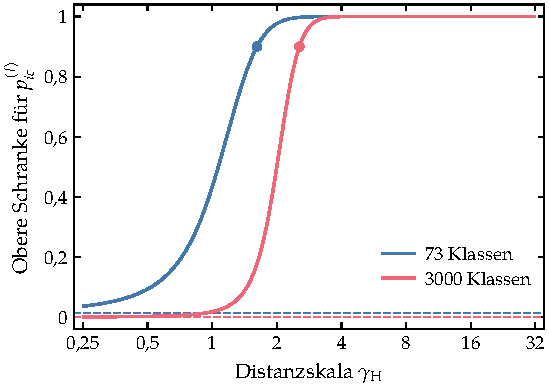
\includegraphics{neu/hoffer_skala}
  \caption[Wirkung der Distanzskala bei der Entropieminimierung nach Hoffer und Ailon]{Obere Schranke der Zuordnungswahrscheinlichkeit nach Gleichung~\eqref{eq:hoffer:schranke} über $\gamma_{\mathrm{H}}$ für 73 bzw.\ \num{3000} bekannte Klassen, etwa die Klassenzahlen eines Cars196- bzw.\ In-Shop-Folds bei Labels in jeder Klasse. Gestrichelt: Gleichverteilung $1/C_{\mathrm{L}}$. Punkte: notwendige Mindestskala für $p^{(l)}_{ic}=0{,}9$.}
  \label{fig:hoffer:skala}
\end{figure}

Die Entropieminimierung nach Hoffer und Ailon wird \ac{SERAPH} und \ac{ISMLP} vorgezogen, weil sie nur Embeddings und gelabelte Referenzbilder braucht und daher mit allen fünf Verlustfunktionen auf dieselbe Weise kombiniert werden kann. 

\ac{SERAPH} würde eine Auswahl ungelabelter Paare, eine Distanzschwelle und eine Übertragung der Spurregularisierung erfordern. Gegen \ac{SERAPH} spricht außerdem der Rechenaufwand, da das Verfahren nur langsam konvergiert~\cite{dutta_semi-supervised_2021} und eine Suche mit vielen Läufen damit teurer wird. \ac{ISMLP} benötigt Proxys, die, zumindest für paarbasierte Verlustfunktionen, zusätzlich ermittelt werden müssen. Beide Verfahren wurden in den Vorexperimenten erprobt (Abschnitt~\ref{sec:e:phase0}). Die Wahl begründet keine allgemeine Überlegenheit dieses Verfahrens. Ein einzelnes Referenzbild kann die Streuung einer Klasse nur eingeschränkt vertreten. Die Implementierung ist jedoch deutlich leichter und repräsentiert die Entropieminimierung ähnlich wie die anderen Verfahren. 

\subsection{\acs{SLADE}}
\label{sec:m:slade}
\ac{SLADE} wird als clusterbasierter Mechanismus umgesetzt. Alle $n_{\mathrm{T}}$ Epochen bettet der aktuelle Head die ungelabelten Bilder ein und teilt sie mit $k$-Means in so viele Cluster, wie es ein gesuchtes Verhältnis zur Zahl der gelabelten Klassen vorgibt. Bis zur nächsten Neuberechnung bleiben die Cluster fest. Basis $\bm{W}_a$, Verteilungsverlust (Gleichung~\eqref{eq:slade-sd}) und die Auswahl sicherer Paare folgen dem Originalverfahren~\cite{duan_slade_2021}. Die sicheren ungelabelten Paare gehen in dieselbe Verlustfunktion ein wie die gelabelten Bilder. Bei ArcFace und Proxy-Anchor ist das nicht möglich, weil deren Klassenparameter nur die gelabelten Klassen kennen und keine Paare aus unbekannten Clustern verarbeiten können (Abschnitt~\ref{sec:verluste:proxy}). Für diese beiden Verlustfunktionen gehen die sicheren Paare deshalb in einen Contrastive Loss nach Gleichung~\eqref{eq:contrastive} ein, wie in der ursprünglichen Arbeit, dessen Margen gesucht werden. Die Gewichte $w_{\mathrm{reg}}$ und $w_{\mathrm{basis}}$ aus Gleichung~\eqref{eq:slade} werden über eigene Zielverhältnisse $\eta$ und $\eta_{\mathrm{basis}}$ nach Abschnitt~\ref{sec:m:gewicht} bestimmt.

Im Original bildet ein eigens trainierter Teacher die Cluster, aus denen ein Student lernt, der den Teacher anschließend nach dem in Abschnitt~\ref{sec:ssdml} beschriebenen Schema ablöst~\cite{duan_slade_2021}. In dieser Arbeit wird kein getrennter Teacher verwendet. Die Cluster stammen vom selben linearen Head, der danach ohne Zurücksetzen der Gewichte oder des Optimierers weitertrainiert wird. Als Teacher dient nur der Head zum Zeitpunkt der letzten Neuberechnung und das Intervall $n_{\mathrm{T}}$ heißt in den Suchräumen deshalb Teacher-Aktualisierung (Anhang~\ref{sec:anhang:phase1}). Wie bei Noisy Student (Abschnitt~\ref{sec:teacher-student}) wird der Teacher damit periodisch durch den Student ersetzt~\cite{xie_self-training_2019}. Anders als dort wird dafür aber kein neues Modell trainiert. Bei $n_{\mathrm{T}}=1$ werden die Cluster wie die Pseudo-Labels von \ac{LP} und der Graph von \ac{LRML} in jeder Epoche aus den aktuellen Embeddings neu gebildet und vom Teacher-Student-Schema bleibt nur, dass die Ziele innerhalb einer Epoche fest sind.

Diese Umsetzung folgt aus dem Versuchsaufbau. Ein getrennter Teacher wäre wie der Student ein linearer Head auf denselben festen Merkmalen. Ein Self-Training aus mehreren vollständigen Trainingsläufen nacheinander würde zudem die Laufzeit vervielfachen. So berechnet \ac{SLADE} seine Ziele wie \ac{LP} und \ac{LRML} innerhalb eines einzigen Trainings aus dem aktuellen Head neu und bleibt mit ihnen vergleichbar. Mit dem Original teilt diese Variante die Idee, aus Clustern sichere Paarrelationen abzuleiten, nicht aber die Umsetzung als Self-Training. Die ursprüngliche Implementierung wird nicht übernommen, weil ein weitergereichter Teacher Labels aus vorherigen Folds gesehen hätte, die dann zur Validierung verwendet werden. Das wäre Leakage und würde die Validierungsleistung verzerren. 

\section{Training}
\label{sec:training}

Die Skalierung auf $224\times224$ Pixel erfolgt bilinear und ohne Zuschnitt. Nicht quadratische Bilder werden dadurch verzerrt, bleiben aber vollständig sichtbar.

Optimiert wird mit Adam ohne Weight Decay~\cite{kingma_adam_2015}. Verlustfunktionen mit eigenen Klassenparametern (Proxy-Anchor, ArcFace) erhalten einen eigenen Optimierer mit eigener, gesuchter Lernrate und beide Optimierer werden in jedem Schritt aktualisiert. In einer Epoche wird auf so vielen Trainingsbildern trainiert, wie der vollständige Trainingspool des Folds enthält, unabhängig vom Label-Budget. Dadurch ist die Zahl der Optimierungsschritte je Epoche für alle Budgets gleich.

Die \ac{SPC} beträgt 4 für Cars196 und \ac{CUB}, 2 für In-Shop und Semi-iNat-2021 und 8 für die In-Shop-Serie mit gelabelten Klassen. Die Werte sind je Datensatz fest und für alle Verlustfunktionen gleich. Es wird nur die Batchgröße gesucht. Eine größere \ac{SPC} ist auf In-Shop und Semi-iNat-2021 nicht möglich, weil beim kleinsten Budget $k=2$ jede Klasse nur zwei gelabelte Bilder hat. Auf Cars196 und \ac{CUB} beträgt das kleinste Budget $k=4$, sodass dort \ac{SPC}-4 möglich ist. Diesen Wert verwendet eine Vergleichsstudie bei Embedding Losses~\cite{musgrave_metric_2020}. Erst damit sind dort auch Batches mit 256 Bildern möglich, denn bei \ac{SPC}-2 wären dafür 128 Klassen nötig, beim Training stehen je Durchlauf der Kreuzvalidierung aber höchstens 80 Klassen zur Verfügung. Außerhalb ihrer Versuche zum Sampling (Abschnitt~\ref{sec:sampling}) wird in zwei weiteren Vergleichen für alle Verlustfunktionen ebenfalls eine einheitliche \ac{SPC} verwendet, \ac{SPC}-2~\cite{roth_revisiting_2020} bzw.\ \ac{SPC}-4~\cite{berton_all_2025, musgrave_metric_2020}.

Nach jeder Epoche wird auf dem vollständigen Validierungsfold ausgewertet. Behalten wird das Modell der Epoche mit der besten Validierungs-\ac{MAP@R}. Alle Angaben nach dem Training beziehen sich auf dieses Modell und nicht auf die letzte Epoche. Das Training endet, wenn sich die Validierungs-\ac{MAP@R} innerhalb der Patience (Abschnitt~\ref{sec:modellauswahl}) nicht verbessert. Die Patience ist für alle Verfahren gleich und beträgt auf Cars196, \ac{CUB} und In-Shop 20 Epochen und auf Semi-iNat-2021 zehn. Abweichend davon verwenden die Wiederholungen mit fünf Seeds auf \ac{CUB} für alle Verfahren eine Patience von 40 Epochen, weil ein Training dort wenig Rechenzeit benötigt. 





Für jeden Fold wird geprüft, ob die Patience das Training zu früh beendet, weil die Validierungs-\ac{MAP@R} nach einem anfänglichen Einbruch zu langsam wieder steigt. Jeder Lauf mit mindestens einem solchen Fold wird zusätzlich mit verzögerter Patience trainiert, bei der die ersten 20 Epochen nach dem Warm-up keine Patience verbrauchen. Damit alle Läufe eines Vergleichs gleich trainiert werden, berichtet die Arbeit für jeden Lauf die Variante ohne Verzögerung. Das Kriterium, die Ausnahmen und die Werte mit Verzögerung stehen in Anhang~\ref{chap:anhang:verzoegerung}.

\section{Ablauf der Untersuchung}
\label{sec:phasen}	

Der Untersuchung gehen explorative Vorexperimente voraus. In ihnen werden Verfahren und Varianten erprobt und an ihnen orientieren sich die Suchräume der anschließenden Hyperparameteroptimierung. Die Untersuchung selbst gliedert sich in zwei Phasen. Phase~1 bestimmt für jede Kombination die beste Konfiguration und wiederholt diese mit fünf Seeds über alle Budgets. Phase~2 untersucht mit gezielten Eingriffen und Analysen, worauf die Ergebnisse der Phase~1 beruhen.

\subsection{Vorexperimente}
\label{sec:m:phase0}


In den Vorexperimenten werden für die Kombinationen aus Datensatz, Mechanismus und Verlustfunktion 50 Konfigurationen zufällig gezogen und mit höchstens 500 Epochen trainiert. Mechanismen mit mehreren Varianten werden überwiegend in einer Basisvariante untersucht und daneben werden \ac{SERAPH} und \ac{ISMLP} als alternative entropiebasierte Verfahren getestet. In der Basiskonfiguration schließen die Bereiche für die Marge und die Skala von ArcFace, für die Parameter des \ac{MS} Loss mit Miner und für die Temperatur von \ac{NT-Xent} die Werte ein, die eine veröffentlichte Suche auf Cars196 und \ac{CUB} als beste ergab~\cite{musgrave_metric_2020}. Die Bereiche aller Verlustfunktionen enthalten zudem die Standardwerte der Bibliothek~\cite{musgrave_pytorch_losses_code_2026}. Für \ac{SLADE} ist der Bereich der Temperatur $\tau$ enger gefasst und schließt die in dieser Suche ermittelten Werte nicht ein, da der Gradient dort zu klein wird (Tabelle~\ref{tab:first-run-hyperparameter-spaces}). Von den dort aufgeführten Hyperparametern werden die beiden Lernraten, die Skalen $\gamma$ von ArcFace, Circle und Proxy-Anchor, $\gamma^{-}$ des \ac{MS} Loss und $\gamma_{\mathrm{H}}$ von Hoffer, die Temperatur $\tau$ von \ac{NT-Xent} und das Varianzgewicht $w_v$ von \ac{SLADE} logarithmisch gezogen, sodass jede Größenordnung gleich stark vertreten ist. Diese Wahl entspricht einer Empfehlung für Hyperparameter, die nur nach unten begrenzt sind~\cite{bischl_hyperparameter_2023}. 

Nach den Vorexperimenten werden die Grenzen der Suchräume anhand der Verteilung der Versuche über jeden Parameter angepasst. Dazu wird für jeden Versuch sein Rückstand auf den besten Versuch derselben Suche betrachtet. Als gut gilt ein Versuch, der bis auf einen Prozentpunkt an den besten heranreicht. Häufen sich gute Versuche an einer Grenze, könnte das Optimum außerhalb des Bereichs liegen und er wird in diese Richtung erweitert. Enthält ein Randbereich viele Versuche, aber kaum gute, wird er entfernt. Verteilen sich die guten Versuche über den ganzen Bereich, bleibt er unverändert. Für die Lernrate von Circle, \ac{MS} und \ac{NT-Xent} wird ein gemeinsamer niedriger Bereich gewählt, damit Unterschiede zwischen den drei paarbasierten Verlustfunktionen nicht auf verschiedene Suchräume der Lernrate zurückgehen. Das gilt auch für \ac{NT-Xent}, obwohl dort auch hohe Lernraten gute Versuche erreichen, denn der niedrige Bereich enthält für die \UEBL, \ac{LP} und \ac{LRML} ebenfalls gute Versuche, für Hoffer nicht (Abschnitt~\ref{sec:e:phase0}). Cars196 und In-Shop werden gemeinsam beurteilt, \ac{CUB} und Semi-iNat-2021 jeweils für sich. Die Grenzen beruhen damit auf einer Beurteilung der Verteilungen und nicht auf einer festen Regel.

\subsection{Phase 1: Hyperparameteroptimierung und Wiederholungen}
\label{sec:m:phase1}
Für jede Kombination sucht Phase~1 mit Optuna in 80 Versuchen. Zuerst werden 40 Konfigurationen zufällig gezogen, dann schlägt der \ac{TPE} 40 weitere vor~\cite{bergstra_algorithms_2011}. Verwendet wird die multivariate Variante aus Optuna~\cite{watanabe_tree-structured_2023}. Die 80 Versuche sind mehr als die 50 Iterationen bayesscher Optimierung in einer früheren Untersuchung~\cite{musgrave_metric_2020}, weil die \ac{SSL}-Mechanismen zusätzliche Hyperparameter haben. Die 40 zufälligen Versuche geben dem \ac{TPE} einen breiten Ausgangspunkt und dienen später als Stichprobe für die Sensitivitätsanalyse. Zielgröße ist die Validierungs-\ac{MAP@R}, gemittelt über die Folds. Die Versuche der Suche trainieren mit höchstens 600 Epochen, die Testevaluationen mit höchstens \num{1000}. Gesucht werden je nach Mechanismus 3 bis 17 Hyperparameter (Anhang~\ref{sec:anhang:phase1}). Bei \ac{LP} sind es 9 bis 12, bei \ac{SLADE} 13 bis 17 gegenüber 3 bis 6 bei der \UEBL (Tabelle~\ref{tab:phase1:hpo-protokoll}). Die beste Konfiguration wird unverändert auf alle Budgets übertragen und mit fünf Seeds wiederholt. Die Übertragung von einem Budget auf alle ist eine Vereinfachung. Ein Teil der Budgetabhängigkeit kann daraus entstehen, dass eine Konfiguration nur für $k=16$ (In-Shop: $k=2$) ausgewählt wurde und ein Mechanismus mit anderen Hyperparametern bei einem anderen Budget besser abschneiden könnte. 

\subsection{Phase 2: Ablationen}
\label{sec:m:phase2}

In Phase~2 wird untersucht, \emph{warum} ein Mechanismus hilft. Eine Erklärung gilt als gestützt, wenn eine gezielte Änderung des vermuteten Mechanismus die Retrieval-Leistung in die erwartete Richtung verschiebt. Eine Korrelation allein genügt nicht. Die Eingriffe und die erwarteten Richtungen wurden vor den Läufen festgelegt (Tabelle~\ref{tab:phase2:eingriffe} in Anhang~\ref{chap:anhang:phase2}).


Die Ablationen laufen auf Cars196 bei $k=16$ und $k=8$ sowie auf In-Shop bei $k=2$. Dabei ist $k=16$ das Budget der Hyperparametersuche, bei $k=8$ bleibt mehr Raum für Verbesserungen, weil die Mechanismen in Phase~1 dort mehr gewinnen als bei $k=16$. Jede Variante verwendet die Phase-1-Konfiguration mit Seed~2 und ändert nur die genannte Einstellung, sodass die Befunde für die Umgebung dieser Konfiguration gelten. Die Varianten laufen mit einer Grenze von \num{1000} Epochen. Da jede Variante je Budget nur einmal läuft, gilt ein Unterschied erst dann als Befund, wenn er deutlich größer ist als die Streuung zwischen zwei Seeds. Für zwei Läufe mit derselben Seed-Standardabweichung $\sigma$ aus den Phase-1-Wiederholungen beträgt die Standardabweichung ihrer Differenz bei vernachlässigter Kovarianz $\sqrt{2}\,\sigma$. Als Rauschschwelle dient das Doppelte davon, $2\sqrt{2}\,\sigma$, was bei unabhängigen, normalverteilten Läufen etwa einem zweiseitigen Niveau von \qty{5}{\percent} entspräche. Die tatsächliche Streuung der Differenz bestimmt diese Schwelle nicht, weil die Läufe ihren Seed teilen und die Varianz einer veränderten Variante nicht eigens geschätzt wird. Die Rauschschwelle dient der Einordnung, nicht einem kalibrierten Signifikanztest. Je nach Mechanismus und Verlustfunktion sind das 0,3 bis \num{1,1}~Prozentpunkte auf Cars196 bei $k=16$ und 0,1 bis \num{1,4}~Prozentpunkte auf In-Shop. Bei dem Vergleich mit der \UEBL tritt an die Stelle von $\sqrt{2}\,\sigma$ die Wurzel aus der Summe der Seed-Varianzen beider Konfigurationen, ebenfalls unter Vernachlässigung der Kovarianz. Wenn alle fünf Verlustfunktionen vorliegen, wird zusätzlich angegeben, ob ein Unterschied mit allen fünf dasselbe Vorzeichen hat. Eine solche einheitliche Richtung wird als Hinweis berichtet, auch wenn einzelne Unterschiede unter der Rauschschwelle bleiben. Als Befund gilt ein Unterschied aber nur für die Verlustfunktionen, bei denen er die Rauschschwelle übersteigt. Für die Concat-\ac{MAP@R} wird die Rauschschwelle auf dieselbe Weise aus der Seed-Standardabweichung der Concat-\ac{MAP@R} der Phase-1-Wiederholungen bestimmt. Bei $k=8$ stammen die Rauschschwellen aus den Phase-1-Wiederholungen bei $k=8$.

Neben der im Folgenden beschriebenen $2\times2$-Zerlegung, der Kontrolle mit abgeschaltetem \ac{SSL}-Term und den Oracle-Pseudo-Labels umfasst Phase~2 weitere Eingriffe. Pseudo-Labels bzw.\ Graph werden nach dem Warm-up einmal berechnet und danach nicht mehr erneuert. Der Graph von \ac{LP} und \ac{LRML} wird unter Erhalt der Knotengrade zufällig umverdrahtet~\cite{maslov_specificity_2002}. Mit den verdeckten Labels werden alle Kanten zwischen verschiedenen Klassen entfernt, als Kontrolle dieselbe Zahl zufälliger Kanten. Sweeps variieren je einen Hyperparameter der Phase-1-Konfiguration. Tabelle~\ref{tab:phase2:eingriffe} führt alle Eingriffe mit ihrer Umsetzung und der erwarteten Richtung auf.

Die $2\times2$-Zerlegung soll trennen, ob ein Gewinn von den ungelabelten Bildern oder von den eigens gesuchten Hyperparametern der \ac{SSL}-Konfiguration stammt. Sie kreuzt die Hyperparameter der \UEBL und die der \ac{SSL}-Konfiguration mit dem Training mit und ohne ungelabelte Bilder (Tabelle~\ref{tab:m:2x2}). Zwei der vier Kombinationen liegen bereits vor, die \UEBL selbst und die unveränderte \ac{SSL}-Konfiguration. Für die beiden übrigen wird jede \ac{SSL}-Konfiguration zweimal zusätzlich trainiert. Im ersten Lauf, der Variante mit den Hyperparametern der \UEBL, übernimmt sie für alle Hyperparameter, die beide Suchen optimiert haben, die Werte der \UEBL und behält nur ihre \ac{SSL}-spezifischen Parameter. Im zweiten Lauf, der Variante ohne ungelabelte Bilder, behält sie ihre eigenen Hyperparameter, aber ohne ungelabelte Bilder. Dazu erhält der ungelabelte Strom die gelabelten Bilder ohne ihre Labels, wobei die Zahl der Updates pro Epoche gleich bleibt. Mit den Hyperparametern der \UEBL ist der Lauf ohne ungelabelte Bilder dagegen die \UEBL selbst, in der Term und ungelabelte Bilder gemeinsam fehlen, sodass der Vergleich mit der \UEBL dort beide nicht trennt. In der Zeile der \ac{SSL}-Konfiguration zeigt der Vergleich also den Beitrag der ungelabelten Bilder, in der Spalte mit ungelabelten Bildern den der eigens gesuchten Hyperparameter.
\begin{table}[tbp]
  \centering
  \caption[Kombinationen der $2\times2$-Zerlegung]{Kombinationen der $2\times2$-Zerlegung. Ohne ungelabelte Bilder erhält der \acs{SSL}-Mechanismus statt der ungelabelten die gelabelten Bilder ohne ihre Labels.}
  \label{tab:m:2x2}
  \small\begin{tabular}{@{}l>{\raggedright\arraybackslash}p{5.0cm}>{\raggedright\arraybackslash}p{5.0cm}@{}}
    \toprule
    Hyperparameter & mit ungelabelten Bildern & ohne ungelabelte Bilder \\
    \midrule
    der \UEBL & Variante mit den Hyperparametern der \UEBL & \UEBL selbst \\
    der \acs{SSL}-Konfiguration & \acs{SSL}-Konfiguration aus Phase~1 & Variante ohne ungelabelte Bilder \\
    \bottomrule
  \end{tabular}
\end{table}
Den Beitrag des Terms allein zeigt der Vergleich der Variante ohne ungelabelte Bilder mit der Kontrolle mit abgeschaltetem \ac{SSL}-Term. Beide verwenden die \ac{SSL}-Hyperparameter, ihr Unterschied zeigt also, was der \ac{SSL}-Term bewirkt, wenn er nur die gelabelten Bilder sieht. Ohne vorab festgelegte Erwartung läuft jede \ac{SSL}-Konfiguration außerdem einmal ohne Warm-up.

Für \ac{LRML}, dessen Abstand zwischen Concat und Mean in Phase~1 auf Cars196 beim kleinsten Budget $k=4$ am weitesten über dem der \UEBL liegt, werden die $2\times2$-Zerlegung und die Kontrolle mit abgeschaltetem \ac{SSL}-Term außerdem bei $k=4$ mit allen fünf Verlustfunktionen und den fünf Seeds der Phase~1 trainiert. Dieser Versuch soll zeigen, welche Komponente den zusätzlichen Gewinn im Ensemble trägt. Die Unterschiede werden seedweise gepaart und es wird angegeben, in wie vielen der 25 Paare aus Verlustfunktion und Seed sie dasselbe Vorzeichen haben. Da die Embeddings jedes Heads auf Länge eins normiert werden, ist die Kosinusähnlichkeit zweier Bilder in $\bm{f}^{\mathrm{cat}}$ genau das Mittel ihrer Ähnlichkeiten in den vier Heads. Im Ensemble können sich deshalb nur Fehler wegmitteln, die nicht alle Heads teilen. Als Maß dafür dient der Anteil der falschen Nachbarn unter den ersten $R_q$ Treffern eines Heads, die ein anderer Head für dieselbe Query ebenfalls unter seinen ersten $R_q$ Treffern hat. Gemittelt wird über alle Paare von Heads und jede siebte Query der Testmenge.

In der In-Shop-Serie mit gelabelten Klassen läuft die $2\times2$-Zerlegung für \ac{LRML} außerdem bei \qty{10}{\percent} gelabelter Klassen, dem Anteil der Hyperparametersuche, mit allen fünf Verlustfunktionen und Seed~2. Die ungelabelten Bilder stammen dort ausschließlich aus Klassen ohne Label. Die Variante ohne ungelabelte Bilder zeigt deshalb, ob \ac{LRML} Bilder neuer Klassen verwerten kann. Die Rauschschwellen stammen hier aus den Phase-1-Wiederholungen bei \qty{10}{\percent}.

Die Oracle-Varianten berechnen in jeder Epoche die Pseudo-Labels und die Auswahl der übernommenen Bilder aus ihrem jeweils aktuellen Head. Für die ausgewählten Bilder ersetzen sie die Pseudo-Labels durch die wahren Labels. Eine je Bild fest gezogene Zufallszahl bestimmt, ob sein Label bei einer vorgegebenen Fehlerrate von 0, 10, 20, 40 bzw.\ \qty{60}{\percent} verfälscht wird. Die so entstehende Kurve zeigt, ob reguläres \ac{LP} bei gleicher gemessener Fehlerrate über oder unter den Läufen mit zufälligen Fehlern liegt. Verrauschte Labels wurden auch beim Training von Retrieval-Modellen untersucht, dort aber an den gelabelten Trainingsdaten und nicht an Pseudo-Labels~\cite{berton_all_2025}.

Dabei wurde auf Cars196 und \ac{CUB} auch bei \qty{32}{\percent} zufällig verfälschten Labels eine geringe Rauschempfindlichkeit berichtet~\cite{berton_all_2025}.

\subsection{Externe ungelabelte Bilder}
\label{sec:m:extern}

\ac{SLADE} wurde in einem anderen Setting evaluiert als dem dieser Arbeit. Dort sind alle Bilder der Trainingsklassen gelabelt und die ungelabelten Bilder stammen aus einem externen Datensatz~\cite{duan_slade_2021}. Ein zusätzlicher Versuch überträgt dieses Setting auf alle vier Mechanismen. Auf Cars196 und In-Shop sind alle Bilder der Trainingsklassen gelabelt. Der ungelabelte Pool besteht aus einem Anteil von CompCars bzw.\ Fashion200k (Abschnitt~\ref{sec:daten}). Auf Cars196 werden 10, 25, 50 und \SI{100}{\percent} der \num{16537} Bilder verwendet, auf In-Shop 5, 10, 25 und \SI{50}{\percent} der \num{338340} Bilder. Die Auswahl ist fest, für alle Folds und Mechanismen gleich und geschachtelt, sodass ein größerer Anteil die Bilder jedes kleineren enthält. Bei CompCars verteilt sie sich gleichmäßig über dessen Klassen. Jeder Mechanismus läuft mit allen fünf Verlustfunktionen, Seed~2 und seiner Phase-1-Konfiguration mit höchstens \num{1000} Epochen. Die Hyperparameter wurden also für wenige Labels und den internen Pool gesucht und für dieses Setting nicht neu optimiert. Referenz ist die \UEBL mit allen Labels, ebenfalls mit Seed~2 und ihrer Phase-1-Konfiguration. Als Kontrolle läuft jede \ac{SSL}-Konfiguration außerdem mit allen Labels und ohne externe Bilder. \ac{LP} und \ac{LRML} erhalten dann einen leeren ungelabelten Pool, sodass \ac{LP} keine Pseudo-Labels bildet und der Term von \ac{LRML} nur auf dem Graphen der gelabelten Bilder wirkt. Hoffer und \ac{SLADE} benötigen ungelabelte Bilder und laufen deshalb mit abgeschaltetem \ac{SSL}-Term. Auf Cars196 laufen \ac{LP} und \ac{LRML} zusätzlich bei jedem Anteil mit 50, 100, 200 und 300 Nachbarn und \ac{SLADE} mit einer festen Zahl von 100 bis 500 Clustern statt des Clusterverhältnisses, im Bereich der Clusterzahlen, die für \ac{SLADE} untersucht wurden~\cite{duan_slade_2021}. Ein Unterschied gilt wie in Phase~2 erst oberhalb der Rauschschwelle für den Vergleich mit der \UEBL als Befund (Abschnitt~\ref{sec:m:phase2}).

\subsection{Verfolgung der Embedding-Geometrie}
\label{sec:m:geometrie}
Um zu erkennen, wie die Mechanismen den Embedding-Raum verändern, werden die Phase-1-Konfigurationen\footnote{Für \ac{LRML} verwenden die Geometrieläufe auf Cars196, In-Shop und in der In-Shop-Serie mit gelabelten Klassen die Konfiguration einer Suche, die sich von der in Abschnitt~\ref{sec:m:phase1} nur durch die univariate Variante des \ac{TPE} unterscheidet.} mit Seed~2 für alle 25 Kombinationen trainiert und dabei verfolgt. Auf Cars196 und Semi-iNat-2021 werden alle vier Budgets betrachtet, auf In-Shop $k=2$ und 4. In der In-Shop-Serie mit gelabelten Klassen werden alle vier Anteile betrachtet. Die Geometrieläufe berechnen die Maße aus Abschnitt~\ref{sec:geometrie} nach jeder Epoche auf allen Bildern. Auf Cars196 und auf Semi-iNat-2021 bei $k=16$ wird dieselbe Konfiguration zusätzlich in getrennten Graphläufen trainiert. Die Graphläufe halten für eine feste Auswahl von 4000 Bildern des Trainingspools die Embeddings und den \ac{kNN}-Graphen fest und speichern die Pseudo-Labels, die \ac{LP} in jeder Epoche übernimmt. Darauf beruhen die Darstellung mit \ac{t-SNE} und die Auswertung der Pseudo-Labels in Abschnitt~\ref{sec:e:pseudolabels}.

Die Maße werden in den Geometrieläufen vor dem ersten Optimierungsschritt (Epoche~$-1$) und danach nach jeder Epoche getrennt für den ganzen Trainingspool, seine gelabelten und seine ungelabelten Bilder, die Validierungs- und die Testklassen berechnet. In den Graphläufen erfolgt die Messung dagegen nur nach jeder fünften Epoche, auf Semi-iNat-2021 nach jeder zweiten. So lässt sich unterscheiden, ob ein Head nur die gelabelten Bilder ordnet oder auch die übrigen Bilder derselben Klassen und ungesehene Klassen. Spektraler Abfall und $\pi_{\mathrm{ratio}}$ werden aus der Referenzimplementierung übernommen~\cite{roth_revisiting_code_2020}. $\pi_{\mathrm{intra}}$, $\pi_{\mathrm{inter}}$ und ihr Verhältnis werden in jeder gemessenen Bildmenge nur über die Klassen berechnet, die dort mindestens zwei Bilder haben, damit das Verhältnis für beide Maße dieselben Klassen beschreibt. $\pi_{\mathrm{inter}}$ und das Verhältnis setzen zusätzlich mindestens zwei dieser Klassen voraus. Bezugspunkt ist neben den DINOv2-Merkmalen der Head vor dem ersten Optimierungsschritt, weil schon die zufällige Projektion das Spektrum verändern kann.

Mit den verdeckten Labels werden außerdem zwei Größen gemessen. Als Prototyp einer Klasse dient der Mittelpunkt der Embeddings ihrer gelabelten Bilder~\cite{snell_prototypical_2017}. Anders als dort, wo der nächste Prototyp nach der quadrierten euklidischen Distanz bestimmt wird, entscheidet hier die Kosinusähnlichkeit. Die Genauigkeit der Prototypen-Zuordnung ist der Anteil der ungelabelten Bilder, deren ähnlichster Prototyp zu ihrer eigenen Klasse gehört. Die Reinheit der Kanten ist der Anteil der Kanten eines \ac{kNN}-Graphen über den Trainingspool zwischen Bildern derselben Klasse. Die Prototypen-Genauigkeit ist für die In-Shop-Serie mit gelabelten Klassen nicht definiert, da die ungelabelten Bilder dort zu Klassen ohne gelabeltes Bild gehören. Die Reinheit wird mit der Nachbarzahl und der Gewichtung des jeweiligen Mechanismus gemessen und für die \UEBL, Hoffer und \ac{SLADE} mit zehn Nachbarn. Sie ist daher nur bei gleicher Graphkonstruktion unmittelbar vergleichbar. 

Für die falschen Pseudo-Labels von \ac{LP} wird gezählt, wie viele ein Modell desselben Herstellers nennen, verglichen mit dem Anteil bei zufälliger Verwechslung. Diese Auswertung beruht auf den tatsächlich im Training übernommenen Pseudo-Labels des ganzen Pools, nicht auf der zusätzlichen Propagation der Graphläufe. Die verfolgten Bilder des Graphlaufs auf Cars196 werden mit \ac{t-SNE} dargestellt~\cite{van_der_maaten_visualizing_2008}. Die Maße nach dem Training stammen in den Geometrieläufen aus der per Validierung gewählten Epoche, in den Graphläufen aus der letzten verfolgten Epoche, die nicht nach ihr liegt. Die Tabellen und die Abbildungen mitteln über die Verlustfunktionen und die vier Folds. Verhältnisse werden dabei je Fold berechnet und erst danach gemittelt, sodass ein Tabellenmittel des Verhältnisses nicht dem Verhältnis der Tabellenmittel entsprechen muss.%


Vorab wurde folgende Erwartung festgelegt: Wenn die ungelabelten Bilder als Regularisierer gegen die Überanpassung an wenige Labels wirken, sollte der Head der \UEBL bei kleinem $k$ stärker komprimieren als die Heads der \ac{SSL}-Mechanismen, erkennbar an einem größeren spektralen Abfall. Der Unterschied sollte mit wachsendem $k$ kleiner werden. Zusätzlich prüft die Arbeit, ob sich der in Abschnitt~\ref{sec:geometrie} beschriebene Zusammenhang zwischen den Geometriemaßen und der Leistung auf ungesehenen Klassen in diesem Setting wiederfindet. Dazu werden die Maße nach dem Training für jede Kombination aus Verfahren, Verlustfunktion und Budget über die vier Folds gemittelt. Die Korrelation mit der Test-\ac{MAP@R} der einzelnen Fold-Modelle wird über alle Kombinationen eines Datensatzes bzw. einer In-Shop-Serie und innerhalb jedes Budgets berechnet. Grundlage dafür ist, wie im ursprünglichen Vorgehen~\cite{roth_revisiting_2020}, der Trainingspool. Weil die ungelabelten Bilder des Pools für die \ac{SSL}-Mechanismen aber Trainingsdaten sind und für die \UEBL nicht, wird die Korrelation zusätzlich auf den Validierungs- und den Testklassen berechnet, deren Bilder in keinen Gradientenschritt eingehen.


\subsection{Sensitivitätsanalyse der Hyperparameter}
\label{sec:m:sensitivitaet}

Zusätzlich werden die vorhandenen Versuche der
Vorexperimente und der Phase~1 ausgewertet, ohne neue
Läufe durchzuführen. Für die zufällig gezogenen
Konfigurationen der Phase~1 (Abschnitt~\ref{sec:modellauswahl}) wird für jeden numerischen
Hyperparameter die Rangkorrelation nach Spearman mit
der Validierungs-\ac{MAP@R} bestimmt~\cite{spearman_proof_1904}.
In dieser Arbeit hebt sich ein Hyperparameter in einer Suche vom Rauschen ab, wenn diese
Rangkorrelation zweiseitig auf dem Niveau von \qty{5}{\percent} von null verschieden ist.

Als deskriptives Maß für die Häufigkeit nahezu
optimaler Konfigurationen werden die Anzahl und der
Anteil der Versuche bestimmt, deren Validierungs-\ac{MAP@R}
höchstens einen Prozentpunkt beziehungsweise einen
Standardfehler der Fold-Werte unter dem besten
Ergebnis liegt.

\subsection{Messung von Rechenzeit und Speicherbedarf}
\label{sec:m:aufwand}

Die Läufe der Hyperparametersuche und der Wiederholungen liefen parallel und bei wechselnder Auslastung auf geteilten \acp{GPU}, sodass ihre Laufzeiten nicht vergleichbar sind. Stattdessen wird auf In-Shop bei $k=2$ für jede Kombination aus Verfahren und Verlustfunktion die in Phase~1 gewählte Konfiguration mit einer Batchgröße von 128 für einen Fold allein auf einer H100-\ac{GPU} trainiert, bei \ac{LRML} eine Konfiguration aus einer anderen Suche mit derselben Verlustfunktion. Gemessen werden nach dem Warm-up die mittlere Dauer eines Trainingsschritts und die mittlere Dauer einer Epoche, einschließlich der Neuberechnung des Graphen, der Pseudo-Labels oder der Cluster und der Validierung. Berichtet wird der Median über die fünf Verlustfunktionen. Die Dauer eines Folds ergibt sich aus den Raten, die bei der Batchgröße des jeweiligen Phase-1-Folds gemessen wurden (Batchgrößen 32 bis 512), dessen Warm-up und der Zahl seiner trainierten Epochen. Berichtet wird der Median über die 100 Folds je Verfahren aus fünf Verlustfunktionen, fünf Seeds und vier Folds.

Der Speicherbedarf der Verlustfunktionen hängt nicht vom Bildinhalt ab und wird deshalb mit zufälligen Merkmalen bestimmt. Gemessen wird der Spitzenwert des zusätzlich belegten \ac{GPU}-Speichers gegenüber dem Zustand vor einem Trainingsschritt.
